\chapter{Introduction to the SSFM for vortex simulations}
\label{ch:splitop}

The Split-Step Fourier Method (SSFM) is a pseudo-spectral technique for solving partial differential equations and is particularly useful for NonLinear Scr\"odinger Equations (NLSEs), such as the Gross--Pitaevskii Equation (GPE),

$$
i \hbar \frac{\partial \Psi(\mathbf{r},t)}{\partial t} = \left(\frac{p^2}{2m} + V_0 + g |\Psi(\mathbf{r},t)|^2 \right)\Psi(\mathbf{r},t)
$$

\noindent where $\mathbf{r}$ is a position vector, $\Psi(\mathbf{r},t)$ is a many-body quantum wavefunction, $p = -i\hbar\nabla$ is the momentum operator, $V_0$ is the trapping potential, g = $\frac{4\pi\hbar^2 a_s}{m}$ is the interaction strength, $a_s$ is the scattering length of the atomic species, and $m$ is the mass.
This equation along with all of its ramifications will be described fully in this chapter.
By solving the GPE with time, we can determine the dynamics of Bose--Einstein Condensates (BECs), and
the states found with the GPE are virtually identical to those found in experiments.

To begin, we will build up the intuition for the GPE from the ground-up, starting with a discussion of the Schr\"odinger equation and the Hamiltonian.

\section{The Schr\"odinger equation and the Hamiltonian}

\jrs{Intro to 2nd quantization...}

Quantum particles are often described by their wavefunction, $\Psi(\mathbf{r},t)$, where $\mathbf{r}$ is a position-space variable and $t$ is time.
This does not have a simple physical interpretation; however, the wavefunction density, $|\Psi(\mathbf{r},t)|^2$, can be interpreted as a probability distribution in position-space, where peaks represent areas where quantum particles are likely to be found.
As with most probability distributions,

\begin{equation}
    \label{eqn:norm}
    \int_\infty^\infty |\Psi(\mathbf{r},r)|^2 d\mathbf{r} = N,
\end{equation}

\noindent where $N$ is the number of particles in the system.
For certain simulations with SSFM, it is important to ensure the quantum system is normalized correctly and Equation~(\ref{eqn:norm}) is used for this purpose.
As this operation requires a summation, it is not well-optimized for GPU hardware; however, it is possible to perform a parallel reduction, which allows for a considerable improvement on massively parallel systems~\cite{harris2007}.
Even so, the normalization is still a slow operation and should be used sparingly.

For the purposes of this body of work, we can simulate the dynamics of a quantum system by solving the Schr\"odinger equation,

\begin{equation}
    i\hbar\frac{\partial\Psi(\mathbf{r},t)}{\partial t} = \left(\frac{p^2}{2m} + V_0\right) \Psi(\mathbf{r},t)
    \label{eqn:schrody}
\end{equation}

\noindent where $m$ is the mass of the atomic system, $p = -i\hbar\nabla$ is the momentum operator, and $V_0$ is the trapping potential.
This is a partial differential equation that relates the change in the wavefunction with time on the left-hand side to physical arguments like momentum and position on the right.
For this reason, the operator on the right-hand side are often described as the \textit{Hamiltonian operator}, 

\begin{equation}
\mathcal{\hat H} = \frac{p^2}{2m} + V_0
\end{equation}

\noindent which noticeably has two separate operators within it: one in momentum-space ($\mathcal{\hat H}_p = \frac{p^2}{2m}$) and another in position-space ($\mathcal{\hat H}_v = V_0$).
The Hamiltonian describes how the quantum system evolves with time, and in this work, we modify the Hamiltonian to match the various quantum systems we would like to simulate.

\begin{figure}

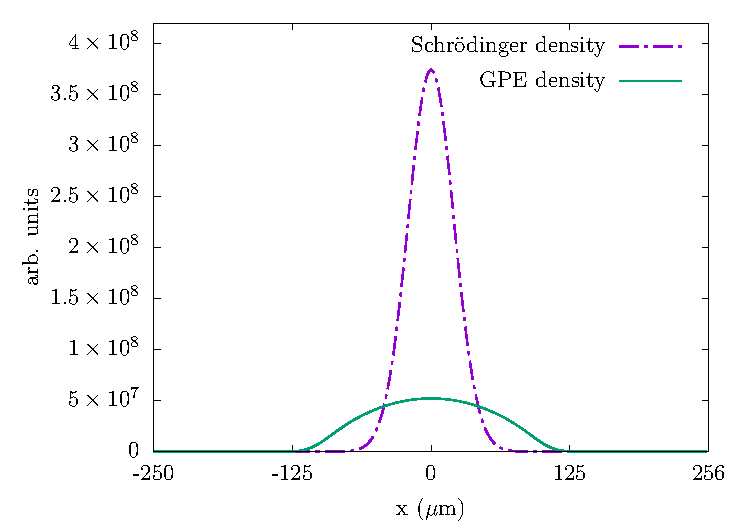
\includegraphics[width = \textwidth]{data/qs/SHO/SHO.pdf}

\caption{Simulated results from ground-state evolution from the split-step Fourier method after 10,000 steps. Here, we use a Rubidium 87 atom with $\omega_x = 1$Hz on a 256-point grid of size 200 $\mu$m. The wavefunction has been normalized such that $\int_{-\infty}^\infty|\Psi|^2 dx = 1$, which provides arbitrary units. We have scaled the potential by $m \omega_x^2 dx^2$ to match these units. This simulation was performed with the GPUE codebase \cite{schloss2018}.}
\label{fig:SHO}
\end{figure}

It is important to note here that the energy of a quantum system is typically described as,

\begin{equation}
\int_{-\infty}^{+\infty}\Psi(\mathbf{r},t)^*\mathcal{\hat H}\Psi(\mathbf{r},t)d\mathbf{r}.
\end{equation}

\noindent Where $\Psi(\mathbf{r},t)^*$ is the Hermitian conjugate of the system.
Often times, this operation is written in \textit{braket} notation like so,

\begin{equation}
\braket{\Psi|\mathcal{\hat H}|\Psi}
\end{equation}

\noindent where the bra ($\bra{}$) operator essentially means that the Hermitian conjugate is required, and the ket ($\ket{}$) means that the vector must remain in whatever space it was in.
Often times, we will describe the wavefunction as a sum of different energy states like so:

\begin{equation}
\Psi = \sum_{n=0}^{\infty}c_n\ket{\psi_n}
\end{equation}

\noindent where $c_n$ is a constant that identifies how much of the wavefunction occupies the state $\psi_n$.
Additionally, we can set the Hamiltonian as a complete set of energy eigenkets, such that $\mathcal{\hat H}\ket{\Psi} = E_n\ket{\Psi}$.

When the quantum system is in its lowest energy state, the probability distribution will often follow the trapping potential.
As an example, consider the case of the simple harmonic oscillator in one dimension, $V_0 = m \omega_x x^2$, where $\omega_x$ is the trapping frequency in the $x$-dimension and describes the tightness of the trap.
In this case, Figure~\ref{fig:SHO} shows the lowest energy state, also called the \textit{ground state} of a quantum system consisting of a single particle.
Notably, the quantum particle rests in the center of the trap and if the trap is moved, the particle will move with it and oscillate about the new trap location.
Many quantum engineering systems require precise control of the trapping potential to manipulate quantum systems~\cite{menchon2016}, and we will discuss two such methods (quantum optimal control~\cite{werschnik2007} and shortcuts to adiabaticity~\cite{guery2019}) in Chapter~\ref{ch:1d}.

\jrs{ADD FIGURE OF OSCILLATION IN REAL-TIME EVOLUTION VIA SEQUENCE.TEX}

Quantum systems do not always have a straightforward interpretation, and $\Psi(\mathbf{r},t)$ is a complex-valued object with operators in both position and momentum space.
As such, it is important to discuss fundamental relationships between position and momentum space in order to better understand quantum systems, and ultimately how the SSFM acts in both spaces.

\section{The Heisenberg uncertainty principle}

\jrs{CN}

The Heisenberg uncertainty principle is a relation between the position and momentum components of a quantum system.
This principle simply states that

$$
\sigma_x \sigma_p \geq \frac{\hbar}{2},
$$

\noindent where $\sigma_x$ and $\sigma_p$ are the standard deviations of the position-space and momentum-space distributions for a quantum system.
Because these two variables are inversely proportional, this can be interpreted to mean that as the measurement in one domain becomes more precise, the measurement in the conjugate domain becomes less so.
This is historically interesting, as it seems to provide the fundamental limit to the precision by which the momentum or position of a quantum particle can be measured to be Planck's constant $h$.

For the purposes of this work, we do not need to delve too deeply into the interpretation of this principle.
Instead, we need to find an appropriate mathematical formalism that allows for us to easily recreate the same properties, and thus develop a method for transforming between position and momentum space for quantum simulations.
In this case, we can see this relation simply by performing a Fourier transform on a set of gaussians with an increasing standard deviation, as shown in Figure~\ref{fig:uncertain}

\begin{figure}

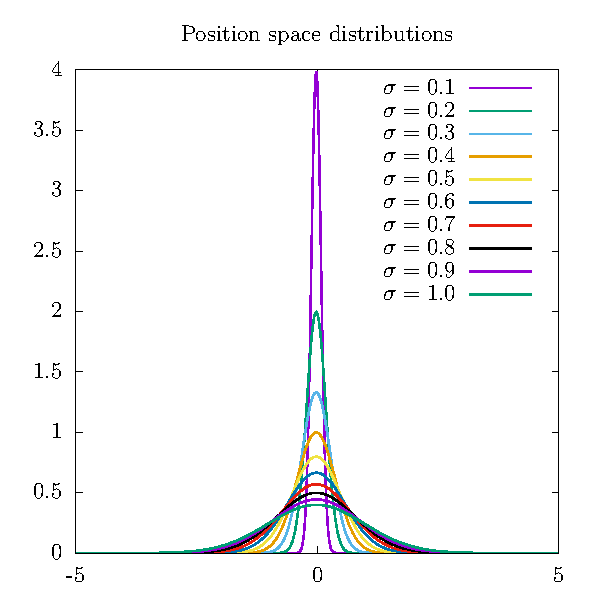
\includegraphics[width = 0.5\textwidth]{data/qs/Heisenberg/position.pdf}
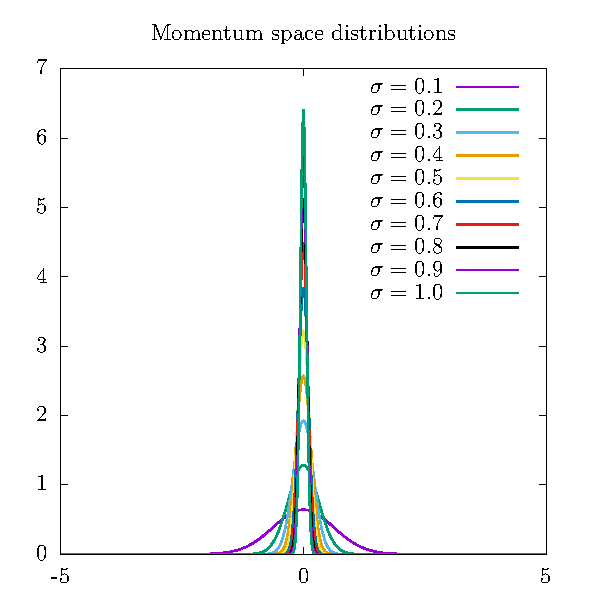
\includegraphics[width = 0.5\textwidth]{data/qs/Heisenberg/momentum.pdf}

\caption{A series of Gaussians with increasing standard deviation. We see that as the standard deviation for the Gaussians in position space increase, the standard devations in momentum space decrease.}
\label{fig:uncertain}
\end{figure}

This indicates that position and momentum are conjugate variables, and 
as such, it is worth exploring the Fourier transform further, as it is also fundamental to the SSFM, itself.

\section{The Fourier transform}

\begin{figure}

\begin{centering}

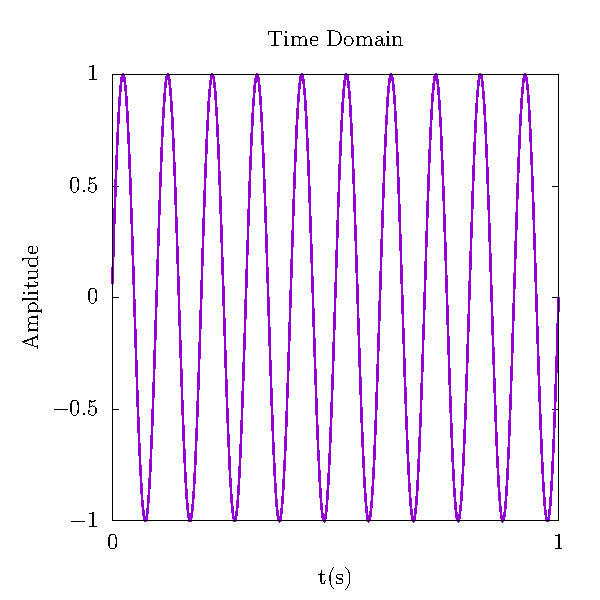
\includegraphics[width = 0.48\textwidth]{data/splitop/fourier/sine_wave.pdf}
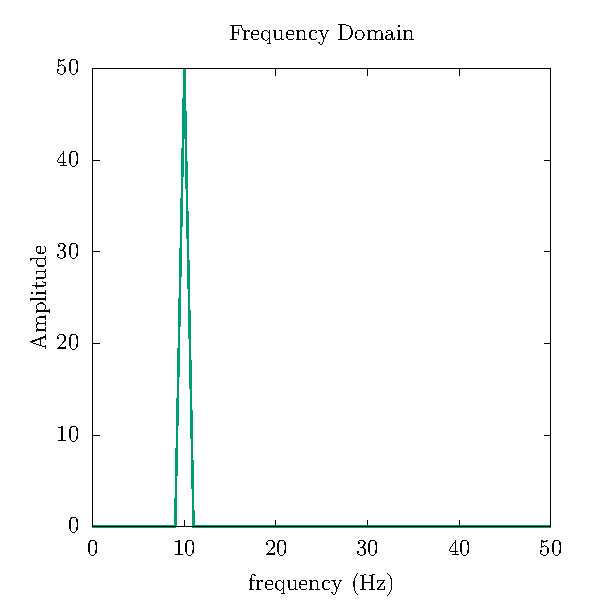
\includegraphics[width = 0.48\textwidth]{data/splitop/fourier/sine_fft.pdf}

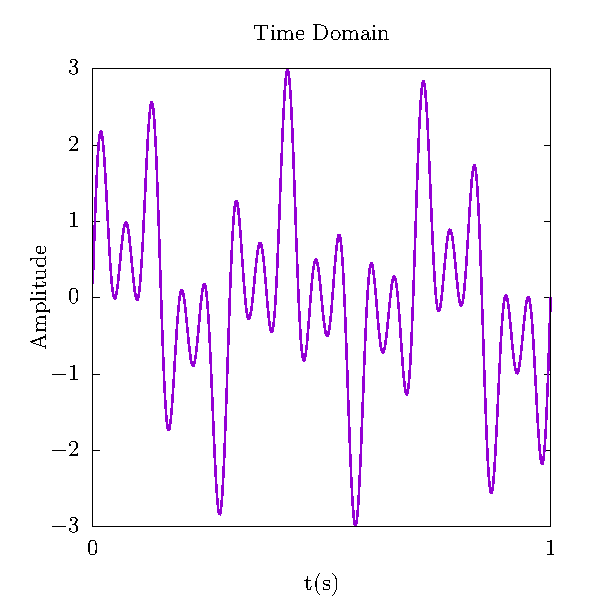
\includegraphics[width = 0.48\textwidth]{data/splitop/fourier/3_waves.pdf}
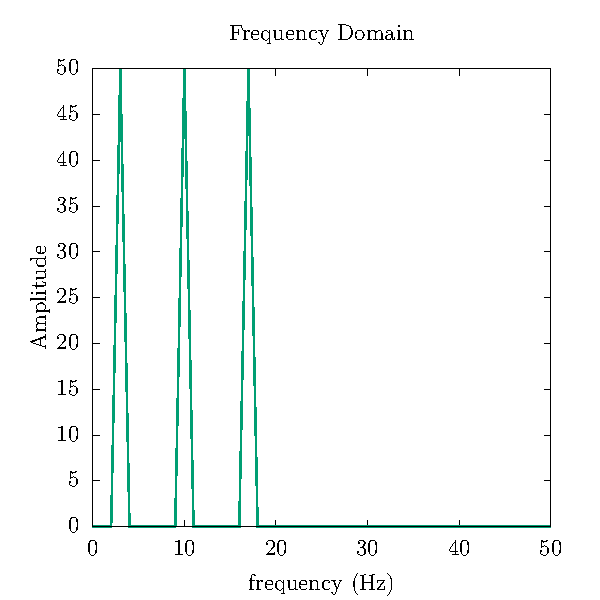
\includegraphics[width = 0.48\textwidth]{data/splitop/fourier/3_fft.pdf}

\end{centering}

\caption{Depiction of a fourier transform, first with a sine wave with a frequency of 10 Hz, and then with a combination of 3 waves of frequencies 3, 10, and 17 Hz. Note that the signal in the Frequency domain is a sparse representation of the singnal in the time domain.}
\label{fig:FT}
\end{figure}

The Fourier transform is a fundamental mathematical technique that lies at the heart of signal processing, and is used for numerous methods, including SSFM.
Because it is such a fundamental technique, there are many intuitive descriptions for interpreting the Fourier transform, and it would not be worthwhile to discuss all of these explanations here.
In most cases, the Fourier transform is introduced as a transformation between the time domain and frequency domain; however, as we discussed in the previous section, it can also transform between any conjugate parameters, such as position and momentum.
As an example, if we have some wave in the time domain with some frequency $\omega$, such as $\sin(20\pi\omega)$, we can plot the signal fully in the time-domain; however, the signal changes to a single peak in the frequency domain, as shown in Figure~\ref{fig:FT}(a).

In fact, every point in the frequency domain corresponds to another distinct wave in the time-domain.
As such, we can decompose most wave-like signals into a sparse set of delta-like peaks in the frequency domain, and this can be seen in Figure~\ref{fig:FT}(b).
In general, if we have a set of parameters that are fully described in one domain, it is likely sparse in it's conjugate domain.
This sparsity has been used for many applications, including compressed sensing, which allows us to reconstruct high-resolution data from low-resolution ouput in a separate domain~\cite{baraniuk2011}.
We will discuss this in more depth in Chapter~\ref{ch:gpue} when we discuss the compressed split-step Fourier method, which applies tecniques in compressive sensing to the SSFM, itself \cite{bayindir2015}.

Mathematically, the Fourier transform can be represented as,

$$
\mathcal{F}(\xi) = \int_{-\infty}^{\infty}f(t)e^{-2\pi i t \xi}dt
$$

\noindent and the inverse Fourier transform can be represented as,

$$
f(t) = \int_{-\infty}^{\infty}\mathcal{F}(\xi)e^{2\pi i t \xi}d\xi
$$

\noindent where $t$ is an element in the time-domain, $\xi$ is an element in the frequency domain, $f(t)$ is a time-domain function, and $\mathcal{F}(\xi)$ is a corresponding frequency-domain function.
In almost all cases related to this work, it is equally important to discuss the Discrete Fourier Transform (DFT), for which the forward transform is,

$$
X_k = \sum_{n=0}^{N-1} x_n e^{-2 \pi i k n / N}
$$

\noindent and the inverse transform is,

$$
x_n = \frac{1}{N} \sum_{k=0}^{N-1} X_k e^{2 \pi i k n / N}
$$

\noindent where $X_k$ and $x_n$ represent the frequency and time domain signals, respectively, $k$ is a component in the frequency domain, $x$ is a component in the time domain, and N is the total number of elements in the signal.
Though the primary difference between these two definitions is that the DFT replaces the integral of the Fourier transform with a sum, the DFT also allows for the computational investigation of signal processing, as it can now be interpreted as a sum and matrix multiplication.
Unfortunately, this comes at a huge cost for complexity, as the matrix multiplication, alone, is of the order of $\mathcal{O}(n^3)$, and with the sum, the DFT has a heafty computational complexity of $\mathcal{O}(n^4)$.

Luckily, there have been several successful attempts to create a Fast Fourier Transform (FFT), including the Cooley-Tukey method, that was first discovered by Gauss and then later contemporized by Cooley and Tukey when they independently discovered it \cite{cooley1965}.
This method is not straightforwardly parallelizable; however, it has become so fundamental to signal processing, that it has become incredibly well-optimized with several libraries, including FFTW~\cite{frigo1998} and CuFFT~\cite{fatica2008} for distributed and GPU calculations, respectively.

\jrs{I want to discuss Cooley-Tukey a bit, but don't know if it's relevant until we talk about parallelization of it.
\begin{itemize}
\item parallelization via CuFFT
\item Justification for DistTrans
\item memory coalescence
\end{itemize}
}

\section{The SSFM}

\begin{figure}

\center 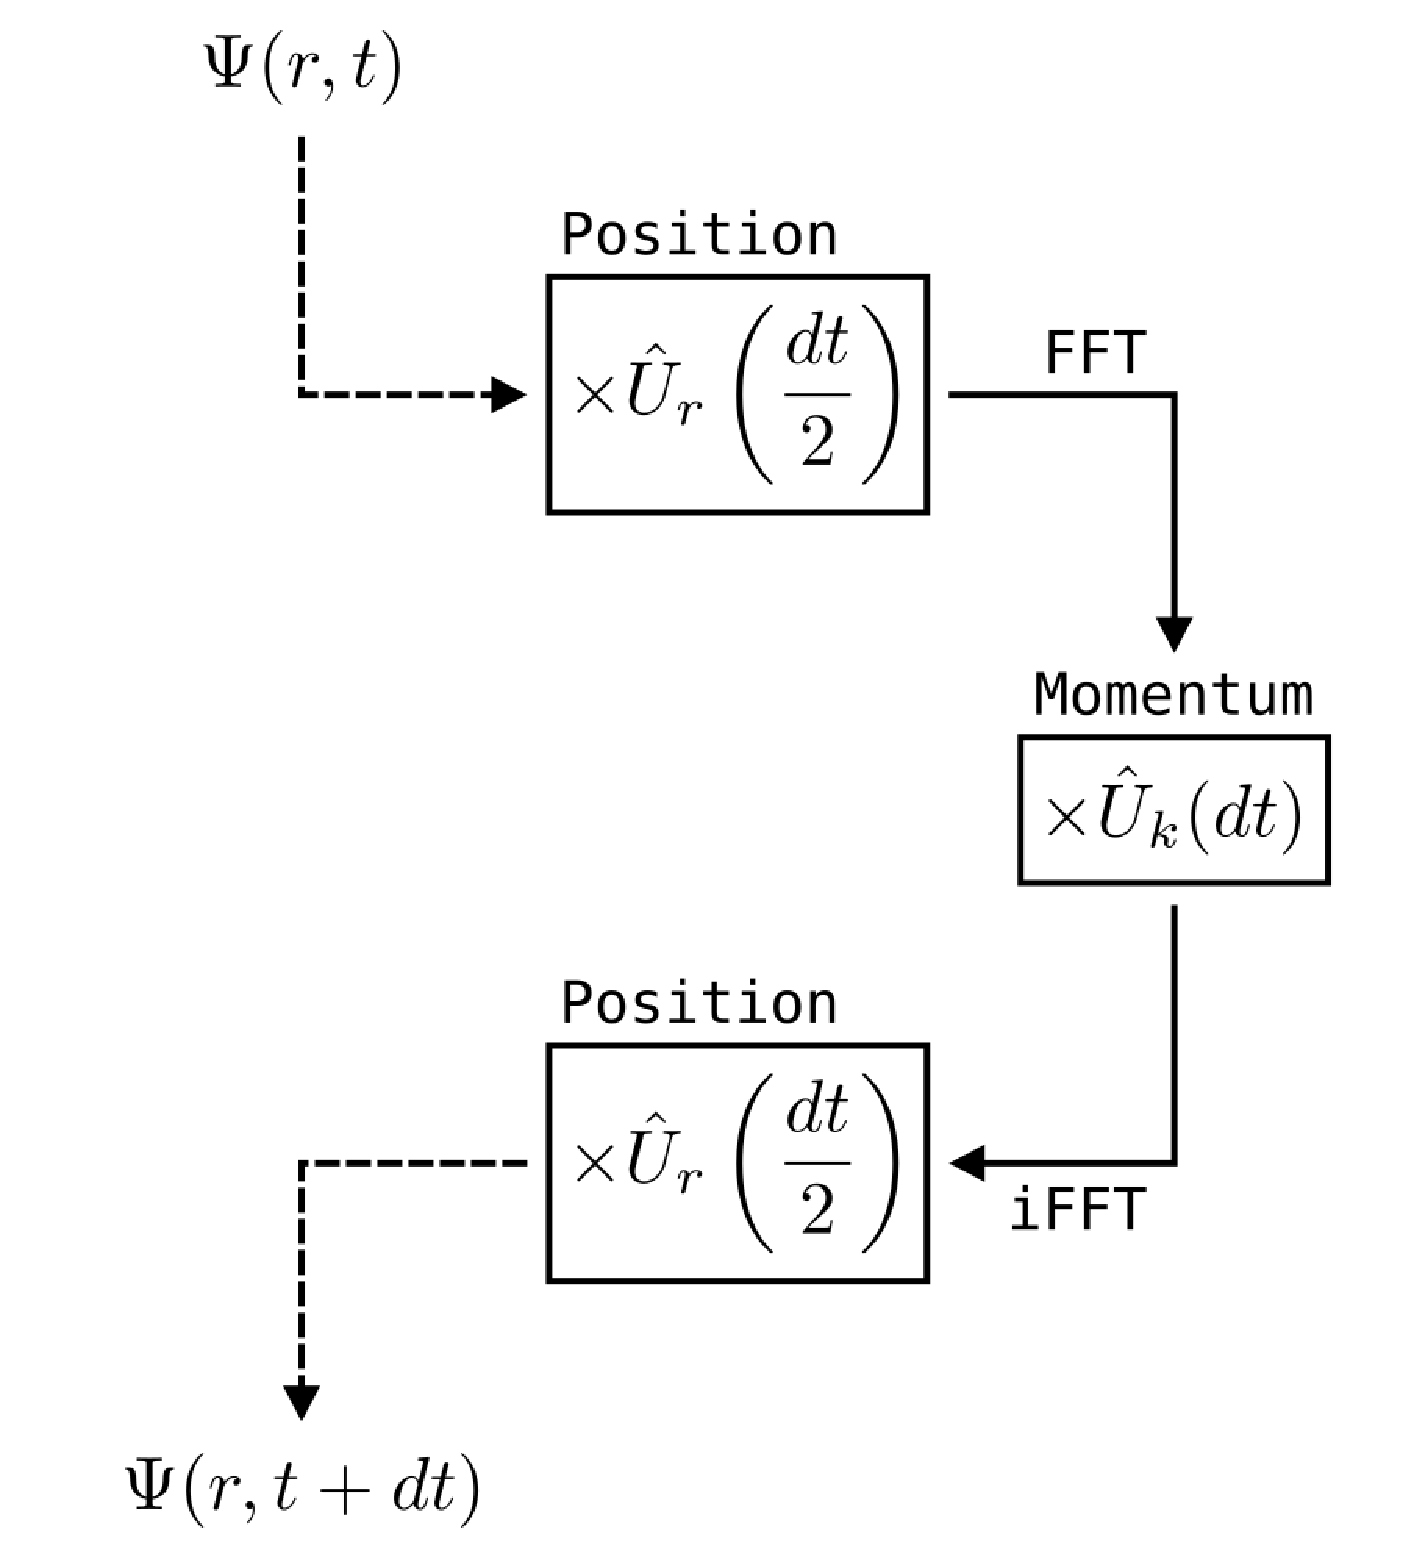
\includegraphics[width=0.5\textwidth]{data/splitop/method/split_op_method.pdf}

\caption{A pictorial representation of the SSFM, created by Julian Schacher~\cite{AAA}.}
\label{fig:method}
\end{figure}

As mentioned, the SSFM splits the Hamiltonian into separate operators and uses the Fourier transform to ensure that these operators work on the wavefunction in the appropriate space.
As discussed, the Hamiltonian operator describes how the quantum system evolves with time.
In order to apply the Hamiltonian to the system, we first assume a somewhat general solution to the Schr\"odinger equation,

$$
\Psi(\mathbf{r},t + dt) = \left[e^{-\frac{i\mathcal{\hat{H}}dt}{\hbar}}\right]\Psi(\mathbf{r},t) = \left[e^{-\frac{i(\mathcal{\hat{H}}_v + \mathcal{\hat{H}}_p)dt}{\hbar}}\right]\Psi(\mathbf{r},t).
$$

\noindent If we assume we are simulating our system by a series of small timesteps ($dt$), we can split this operation by using the Baker-Campbell-Housdorff formula \jrs{CN}:

$$
\Psi(\mathbf{r},t+dt) = \left[e^{-\frac{i\mathcal{\hat{H}}_vdt}{\hbar}}e^{-\frac{i\mathcal{\hat{H}}_pdt}{\hbar}}e^{-\frac{[i\hat{H}_r, i\hat{H}_k]dt^2}{2}}\right]\Psi(\mathbf{r},t)
$$

\noindent This accrues a small amount of error ($dt^2$) related to the third term, which is a commutation of the real and momentum-space components of the Hamiltonian, which is a noticeably high;
However, we can decrease the $dt^2$ error to $dt^3$ by performing a half-step in position space before doing a full-step in momentum space, through a process called \textit{Strang Splitting} like so \jrs{CN}:

$$
\Psi(\mathbf{r},t+dt) = \left[e^{-\frac{i\mathcal{\hat{H}}_vdt}{2\hbar}}e^{-\frac{i\mathcal{\hat{H}}_pdt}{\hbar}}e^{-\frac{i\mathcal{\hat{H}}_vdt}{2\hbar}} \right]\Psi(\mathbf{r},t) + \mathcal{O}(dt^3)
$$

\noindent We can then address each part of this solution in chunks, first in position space, then in momentum space, then in position space again by using Fourier transforms.
Which looks something like this:

$$
\Psi(\mathbf{r}, t+dt) = \left[\hat{U}_r\left(\frac{dt}{2}\right)\mathcal{F}^{-1}\left[\hat{U}_k(dt) \mathcal{F} \left[\hat{U}_r\left(\frac{dt}{2}\right) \Psi(\mathbf{r},t) \right] \right] \right] + \mathcal{O}(dt^3)
$$

where $\hat{U}_r = e^{-\frac{i\mathcal{\hat{H}}_vdt}{2\hbar}}$, $\hat{U}_k = e^{-\frac{i\mathcal{\hat{H}}_pdt}{\hbar}}$, and $\mathcal{F}$ and $\mathcal{F}^{-1}$ indicate forward and inverse Fourier Transforms.
A flowchart of how we perform this operation can be found in Figure~\ref{fig:method} and is essentially composed of the following steps:

\begin{enumerate}
\item Multiply the wavefunction in real space with the real-space operator.
\item Flip to momentum space with a Fourier transform.
\item Multiply the momentum-space wavefuntion by the momentum-space operator.
\item Flip to position space with an inverse Fourier transform.
\item Repeat 1-4 until satisfied.
\end{enumerate}

This will allow for us to simulate the dynamics of a simple quantum system.
For example, if we guess that our initial wavefunction is gaussian-like and is slightly offset from the center or the trap, this should allow us to see our wavefunction sloshing back and forth in our trap, as shown previously in FIGURE \jrs{ADD}.

In addition, we can find the lowest energy state of our system by performing a Wick rotation and using $\tau = it$ for the simulation \jrs{CN}.
This changes the solution from sinusoidal to an exponential decay in the energy,

$$
\Psi(\mathbf{r},\tau + d\tau) = \left[e^{-\frac{\mathcal{\hat{H}}d\tau}{\hbar}}\right]\Psi(\mathbf{r},\tau) = \left[e^{-\frac{(E_n d\tau)}{\hbar}}\right]\Psi(\mathbf{r},\tau)
$$

\noindent In this way, by moving our simulation in imaginary time, we will see an exponential decay of the energy and the wavefunction density until we have converged to the ground state.
As we are interested in the dynamics of the quantum system, every step in imaginary time requires a relatively costly renormalization step via Equation~\ref{eqn:norm}.
A simulation of the same system as in FIGURE, but in imaginary time is shown in FIGURE (a).
In FIGURE (b), we see the energy exponentially decaying to the known ground-state energy of a quantum harmonic oscillator of $\frac{1}{2}\hbar\omega$.

Now we will turn our focus to systems to be simulated via the SSFM throughout this work: ultracold atoms.

\section{Introduction to ultracold quantum systems}
\label{sec:intro}

When atomic systems are cooled to temperatures near absolute zero Kelvin, it becomes easier to discern their quantum properties which vary depending on the system.
Most elementary particles that make up atoms have intrinsic angular momentum known as \textit{spin}.
Electrons are elementary particles with a spin of $\frac{1}{2}$, and protons and nuetrons are made of elementary particles that sum to a spin of $\frac{1}{2}$.
The spin of the entire atom is determined by summing the constituent spin components.
If the sum results in an integer value, the atom is known as a \textit{boson}, and if the sum results in a half-integer value, the atom is known as a \textit{fermion}.

Because fermions have half-integer spin, they must obey the Pauli exclusion principle and are constrained to Fermi--Dirac statistics, which means their ground state will be composed of several fermionic pairs.
This creates a \textit{Fermi sea}, where particles fill defined energy levels from the bottom up with two particles per level.
On the other hand, bosons have integer spin and follow Bose--Einstein statistics.
They will condense into a single, macroscopic ground state when cooled~\cite{Einstein1925, Fetter2003}, and
this state of matter is known as a Bose--Einstein Condensate (BEC).
The BEC has the properties of a superfluid, which will be discussed more completely in the following section.

There are notable exceptions to these rules, such as the highly correlated Tonks--Girardeau gas where bosons may act as spinless, non-interacting fermions \cite{Girardeau}.
Though there also exists a regime where interacting fermions can also condense into a BEC-like system~\cite{Nozieres1985, Bulgac2014}, we will not discuss fermionic systems further in this work.
For now, we will focus on BEC systems, but will also discuss Tonks--Girardeau gas systems later in Chapter~\ref{ch:1d}.


\subsection{Bose--Einstein condensation and the Gross--Pitaevskii Equation}

As mentioned in Section~\ref{sec:intro}, bosons in a BEC condense into the same (ground) state, meaning we must introduce a many-body Hamiltonian for the system and take inter-particle interactions into account.
For the purposes of this body of work, we will only consider two-body interactions and assume any interactions between three or more atoms are unlikely and negligible.
We can write the Hamiltonian with two body interactions in the second quantized form as
\begin{equation}
    \mathcal{\hat H} = \int d\mathbf{r} \hat \Psi^\dagger(\mathbf{r})\left[-\frac{\hbar^2}{2m}\nabla^2 + V_0(\mathbf{r}) \right]\hat \Psi(\mathbf{r}) + \frac{1}{2} \int d\mathbf{r} d\mathbf{r'} \hat \Psi^\dagger(\mathbf{r}) \hat \Psi^\dagger(\mathbf{r'}) V(\mathbf{r} - \mathbf{r'})\hat \Psi(\mathbf{r'}) \hat \Psi(\mathbf{r})
    \label{eqn:2nd}
\end{equation}
where $\mathbf{r}$ and $\mathbf{r'}$ are the positions of the two colliding particles, $V(\mathbf{r}-\mathbf{r'})$ is the interaction potential, and $\hat \Psi^\dagger(\mathbf{r})$ and $\hat \Psi(\mathbf{r})$ are the creation and annihilation operators that follow the commutation relation, $[\hat \Psi(\mathbf{r}),\hat \Psi^\dagger(\mathbf{r})] = \delta(\mathbf{r} - \mathbf{r'})$.

In the case of a BEC at $T\approx0$, we may perform a Bogoliubov expansion~\cite{Bogoliubov1947, Dalfovo1999}
\begin{equation}
    \hat \Psi (\mathbf{r}, t) = \Phi(\mathbf{r},t) + \delta \hat \Phi(\mathbf{r},t)
\label{eqn:bog}
\end{equation}
where $\Phi(\mathbf{r},t) \equiv \langle \hat \Psi(\mathbf{r},t) \rangle$ is the wavefunction of the condensate known as the \textit{order parameter} and $\delta \hat \Phi(\mathbf{r},t)$ represents fluctuations of the BEC system.
In a BEC, the condensate density is defined as
\begin{equation}
    n(\mathbf{r},t) = |\Phi(\mathbf{r},t)|^2.
\end{equation}

Now we may use the Heisenberg equation of motion
\begin{equation}
    i\hbar \frac{\partial}{\partial t}\hat \Psi(\mathbf{r},t) = [\hat \Psi, \hat H]
\end{equation}
    to determine the time evolution of the field operator $\hat \Psi(\mathbf{r},t)$ as
\begin{equation}
    \frac{\partial}{\partial t}\hat \Psi(\mathbf{r},t) = \frac{1}{i\hbar}\left[-\frac{\hbar^2}{2m}\nabla^2 + V_0(\mathbf{r}) + \int d\mathbf{r'} \hat \Psi^\dagger(\mathbf{r'}, t)V(\mathbf{r'} -\mathbf{r})\hat \Psi(\mathbf{r'},t)\right]\hat \Psi(\mathbf{r},t),
\end{equation}
which follows from Equation~\eqref{eqn:2nd} after integrating over $\mathbf{r}$. 
Now we must apply a few approximations for the BEC:
\begin{enumerate}
    \item In the Bogoliubov expansion, Equation~\eqref{eqn:bog}, we assume that $\delta \hat \Phi(\mathbf{r},t)$ is small at $T = 0\text{K}$, and thus $\hat \Psi(\mathbf{r},t) \approx \Phi(\mathbf{r},t)$. 
    \item Two bosons will only interact with a contact potential of the form
    \begin{equation}
        V(\mathbf{r'}-\mathbf{r}) = g\delta(\mathbf{r'} - \mathbf{r}),
    \end{equation}
    which has a strength given by
    \begin{equation}
        g \equiv \frac{4 \pi \hbar^2 a_s}{m},
    \end{equation}
    where $a_s$ is the species and state-dependent s-wave scattering length.
    %\item The bose gas is dilute and the inter-particle spacing is much larger than $a_s$.
\end{enumerate}

With these approximations, we may write the time-dependent Schr\"odinger equation as
\begin{equation}
    i\hbar \frac{\partial}{\partial t}\Phi(\mathbf{r},t) = \left( - \frac{\hbar^2}{2m} \nabla^2 + V_0(\mathbf{r}) + g |\Phi(\mathbf{r},t)|^2\right)\Phi(\mathbf{r},t).
\end{equation}
This equation is known as the nonlinear Schr\"odinger equation due to the presence of the $|\Phi(\mathbf{r},t)|^2$ term.
In the BEC community, the equation is usually called the Gross-Pitaevskii equation (GPE).
When written in the time-independent form it determines the chemical potential $\mu$ of the condensate system~\cite{Gross1961, Pitaevskii1961}
\begin{equation}
    \mu\Phi(\mathbf{r}) = \left( - \frac{\hbar^2}{2m} \nabla^2 + V_0(\mathbf{r}) + g |\Phi(\mathbf{r})|^2\right)\Phi(\mathbf{r},t).
    \label{eqn:GP}
\end{equation}

This equation allows us to determine the full dynamics of a BEC system and the numerical solutions will be discuss in Section~\ref{sec:code}. Similar derivations of the GPE can be found in many introductory texts on BEC physics, such as~\cite{Fetter2003,  Pethick2002, Fetter2009}.


A superfluid is a state of matter that acts like a classical fluid withoug viscosity.
This means that once a superfluid is set in motion, there is no retarding force to keep it from flowing.
There are a few known systems in which superfluidity can exist, such as $^4$He (sometimes called Helium II when in its superfluid phase)~\cite{Allen1938}, neutron stars~\cite{Migdal1960} or BEC systems~\cite{Einstein1925, Anderson1995}.
As stated, we will focus on BEC systems, but it is important to note that any results shown for superfluid vortex dynamics may have applications beyond cold, atomic physics.

Though there are many interesting differences between classical fluids and superfluids, we will focus here on vortex dynamics.
By rotating a fluid, it is possible to create a vortex around the axis of rotation; however, because of the viscosity of a classical fluid, the vortex will begin to shrink and eventually disappear without constant driving.
In a superfluid, this is not necessarily the case.

In addition, due to the quantization of angular momentum in quantum mechanics, the vorticity in a superfluid is also quantized with the circulation defined as~\cite{Pethick2002},
\begin{equation}
\Gamma = \oint\mathbf{v} \cdot d \mathbf{l} = 2\pi \frac{\ell \hbar}{m},
\label{Eq:phase}
\end{equation}
where $\ell$ is an integer value known as the phase winding.
In this case, the velocity is
\begin{equation}
v = \frac{\hbar}{m}\mathbf{\nabla}\phi,
\end{equation}
where $m$ is the mass of the atomic species.
Because the energy $E \propto \ell^2$, as a superfluid is spun faster, a vortex will not grow or shrink in size, but multiple vortices will spawn instead~\cite{Pethick2002}.
In other words, it is energetically favorable for two vortices of smaller angular mementum to form instead of a single vortex with a large amuont of angular momentum.
Large amounts of angular momentum will therefore lead to many vortices, which will arrange themselves in a triangular lattice structure known as an Abrikosov lattice~\cite{Abrikosov1957, Fetter2001}.
This behaviour is identical to that of Type II superconductors under the effects of a magnetic field.

Vortices in superfluid systems are also peculiar in their behaviour when compared to classical vortices.
Superfluid vortices must either end at the end of the condensate or reconnect in the form of vortex rings or other, more complicated vortex structures~\cite{Reichl2013}.
Because the circulation around superfluid vortices is quantized, when two vortices approach each other with different velocity fields, they may reconnect into smaller, more energetically favorable vortex structures.
During this reconnection, the abrupt change in energy will create a sound wave at the reconnection site~\cite{Feynman1955}.

Three dimensional vortex structures have been notoriously difficult to generate in an experimental laboratory... ADD MORE FROM VORTEX STATES PAPER!!!

\section{Methods for vortex generation in superfluid BEC systems}

\subsection{Phase imprinting}
\subsection{Artificial magnetic fields}
\label{sec:gauge}

BECs are typically weakly interacting and composed of neutral atoms, which do not have charge that is directly affected by electric and magnetic fields; however, artificially magnetic fields can still play a crucial role in many cold atomic systems.
For example, artificial magnetic fields can lead to the generation of vortices in BEC systems~\cite{Lin2009}.
Since we desire to generate vortex rings with artificial magnetic fields, a detailed introduction, similar to that given by Dalibard in~\cite{Dalibard2015}, will be presented below.

From classical electrodynamics, we define can the magnetic field as
\begin{equation}
\mathbf{B} = \nabla \times \mathbf{A},
\end{equation}
where $\mathbf{A}$ is known as a vector potential and has no classical physical interpretation.
Thus, it can be be defined somewhat arbitrarily.
For example, if we have a uniform magnetic field in the $\hat z$ direction, $\mathbf{B} = B \hat z$, we may choose from many different options, such as the symmetric gauge
\begin{equation}
\mathbf{A}(r) = \frac{B}{2}(x \hat y - y \hat x),
\end{equation}
or the Landau gauge
\begin{equation}
\begin{split}
\mathbf{A}(r) &= Bx \hat y, \\
\mathbf{A}(r) &= By \hat x.
\end{split}
\end{equation}

Even though $\mathbf{A}$ has no \textit{classical} ramifications, in the \textit{quantum} realm, it can have physical implications.
The most famous example of this is the Aharonov-Bohm effect~\cite{Aharonov1959}. 
Imagine a solenoid extending infinitely in the $\hat z$ direction, with an of electric current circulating through to create a static magnetic field through the center of the solenoid, but not on the exterior. 
As mentioned above, this magnetic field could correspond to a few different gauge choices.
If we send a charged particle from one point on the exterior of the solenoid to an identical point on the other side of the solenoid by avoiding the solenoid, no matter what path we choose to send the particle along, there would be no significant difference between the different chosen paths.
This is obvious because the magnetic field is negligible on the exterior of the solenoid.
If we instead imagine sending a quantum particle around the solenoid, we could imagine a phase associated with a non-zero $\mathbf{A}$ given by
\begin{equation}
\phi = \frac{q}{\hbar}\int_P \mathbf{A} \cdot d\mathbf{r},
\end{equation}
where $q$ is the charge of the particle and $P$ is the chosen path.
If we connect the two paths, then we could imagine a change in phase related to the magnetic flux $\Phi_B = \mathbf{B}\eta$, where $\eta$ is the area within the object. 
That phase difference would be
\begin{equation}
\Delta\phi = \frac{q\Phi_B}{\hbar}.
\end{equation}

The Aharonov--Bohm effect is a simple example with huge consequences: gauge fields matter in quantum mechanics. 
In the following, we will discuss how to use this consequence to our advantage by first rotating our system to generate vortices, and then generating vortices again by using geometric gauge fields.

\subsubsection{Artificial Magnetic Fields With Rotation}
\label{sec:rot}

Even with an appropriate gauge field, to create rotation we still must somehow provide angular momentum to our cold atomic system.
Imagine a charged particle in a magnetic field undergoing gyromotion through the Lorentz force law, $F=q\mathbf{v} \times \mathbf{B}$.
By applying the appropriate transformation, the Hamiltonian for this system becomes
\begin{equation}
\hat H = \frac{(\hat{\mathbf{p}} - q \mathbf{A}(\hat{\mathbf{r}}))^2}{2m} + V_0(\hat{\mathbf{r}}),
\label{eqn:lorentz}
\end{equation}
where $q$ is the charge of the particle and $\hat p$ is its momentum.
Now, let us consider the same law, except with artificial magnetic fields created for cold, atomic systems.

As mentioned before, cold atoms are neutral and because of this, we must find ways to simulate the effects of magnetic fields instead of using magnetic fields themselves.
Imagine a plane rotating with an angular velocity $\Omega$ around the $z$-axis ($\mathbf{\Omega} = \Omega \hat z$). 
In this case, the Coriolis force is defined as
\begin{equation}
\mathbf{F}_{\text{Coriolis}} = 2m \mathbf{v} \times \mathbf{\Omega},
\end{equation}
which is formally similar to the Lorentz force law.
By applying the transformation $\hat H = \hat H_0 - \Omega \hat L_z$, where $\hat L_z = x\partial_y - y\partial_x$, we find~\cite{Bhat2008}
\begin{equation}
\begin{split}
\hat H &= -\frac{\hbar^2}{2m}\nabla^2 + \frac 1 2 m \omega^2(x^2 + y^2) - \frac{\hbar \Omega}{i}(x\partial_y - y\partial_x) \\
 &= \frac{1}{2m}\left(\frac{\hbar}{i}\nabla - m(\mathbf{\Omega} \times \mathbf{r})\right)^2 + \frac m 2 \left( \omega^2 - \Omega^2 \right)r^2 \\
 &= \frac{(\hat{\mathbf{p}}-m\mathbf{A}(\mathbf{r}))^2}{2m}+ V_0(\mathbf{r}),
\end{split}
\end{equation}
where $\omega$ is the trapping frequency for a symmetric two-dimensional harmonic trap, $\mathbf{A} \equiv \mathbf{\Omega} \times \mathbf{r}$, and $V_0 = m/2 \left( \omega^2 - \Omega^2 \right)r^2$.
The final form is similar to that of Equation~\eqref{eqn:lorentz} for the Lorentz force law and coincide with an effective magnetic field according to $2 \mathbf \Omega \rightarrow \mathbf B$.
In this way, we may recreate the rotation expected from the Lorentz force law in a cold atomic system with an artificial magnetic field~\cite{Peshkin1989, Madison2000, Abo-Shaeer2001}.

With this method of generating vortices, the potential term $V_0$ becomes negative when $\Omega > \omega$, which allows particles to exit the trap, and there have been experiments rotating a BEC up to this limit~\cite{Schweikhard2004}.
In 2009, Lin~\textit{et~al.} showed that it was possible to generate vortices with geometric gauge fields instead, which can circumvent this limitation~\cite{Lin2009}.
We will now discuss how to generate vortices in BEC systems with geometric gauge fields instead of rotation.

\subsubsection{Geometric Gauge Fields}
\label{sec:geom}

In the following, we will discuss the adiabatic motion of free atoms undergoing geometric phase transformations through the Berry phase. 
For this, we assume that our system has an external parameter $\lambda$ such that
\begin{equation}
\hat H(\lambda) \ket{\psi_n(\lambda)} = E_n(\lambda)\ket{\psi_n(\lambda)},
\end{equation}
where the set of eigenstates $\left\{ \ket{\psi_n(\lambda)} \right\}$ allow us to define the time evolution of our system such that
\begin{equation}
\ket{\psi(t)} = \sum_n c_n(t) \ket{\psi_n(\lambda(t))},
\end{equation}
and we consider $\lambda$ to evolve slowly with time. If we consider the system to begin with
\begin{equation}
c_l(0) = 1,
\qquad
c_n(0) = 0, 
\qquad
\text{for all } n\neq l
\end{equation}
the state of the system is proportional to $\ket{\psi_l(\lambda(t))}$.
In this case, $c_l(t)$ is determined by the equation
\begin{equation}
i \hbar \dot{c}_l =  [E_l(t) - \dot{\lambda} \cdot \mathbf{A}_l(\lambda)]c_l,
\label{Bcnx-1}
\end{equation}
where 
\begin{equation}
\mathbf{A}_l(\lambda) = i \hbar \braket{\psi_l|\nabla\psi_l}.
\label{eqn:Bcnx}
\end{equation}
This quantity is called the Berry connection, which is considered a vector potential, such that we can define a new artificial magnetic field, the Berry curvature as
\begin{equation}
\mathbf{B}_l = \mathbf{\nabla} \times \mathbf{A}_l.
\label{eqn:BC}
\end{equation}

Now imagine that the $\lambda$ parameter follows the closed contour $C$ such that $\lambda(T) = \lambda(0)$. 
By integrating Equation~\eqref{Bcnx-1} above, we find
\begin{equation}
c_l(t) = e^{i \Phi_{\text{dyn}}(t)}e^{i\Phi_{\text B}(T)}c_l(0),
\label{eqn:c}
\end{equation}
where
\begin{equation}
\begin{split}
\Phi_{\text{dyn}}(T) &= - \frac{1}{\hbar}\int_0^TE_l(t)dt \\
\Phi_{\text{Berry}} (T)&= \frac{1}{\hbar} \int_0 ^T \dot{\lambda} \cdot \mathbf{A}_l(\lambda)dt = \frac{1}{\hbar}\oint\mathbf{A}_l(\lambda) \cdot d\lambda
\end{split}
\end{equation}
In this case $\Phi_{\text{Berry}}$ is called the Berry phase and it only depends on the motion path of $\lambda$. 
It should be mentioned that both of the exponential terms in Equation~\eqref{eqn:c} are gauge invariant and thus remain unchanged when $\ket{\psi_n(\lambda)}$ is multiplied by a phase factor.
This phase allows us to transfer angular momentum into our BEC and generate a vortex geometry like those formed in the 2009 experiment by Lin~\textit{et~al.}~\cite{Lin2009}.
A method to generate these gauge fields in an experimentally realizable way will be described in Section~\ref{sec:evanescent}, but for now let us discuss the possible dynamics of similar in three dimensional systems.

%-------------------------------------------------------------------------------
\section{Vortex ring dynamics in BEC systems}
\label{sec:vortex}

As mentioned in Section~\ref{sec:intro}, in BEC systems with large amounts of angular momentum and a single axis of rotation, the vortices will create a two-dimensional Abrikosov lattice. 
This regular structure is a direct consequence of the quantization of angular momentum in quantum mechanics.
There are many interesting features to vortices in superfluid systems, many of which follow from classical fluid dynamic theory~\ref{Fetter2009}, which is a well-studied field and covered in many texts~\cite{Faber1995, Kundu2012, Tritton1988, Landau1987}
Here, we discuss the dynamics of vortex rings in BEC systems.

In a three dimensional BEC and other superfluid systems, vortices can be described as as a system of freely-moving, current-carrying wires located along the axis of rotation. 
In this way, it is possible to model such systems using the Biot-Savart law ~\cite{Schwarz1985}
\begin{equation}
    \boldsymbol{v}_s(\boldsymbol{r},t) = \frac{\kappa}{4\pi}\int\frac{|s_1-\boldsymbol{r}|\times ds_1}{|s_1-\boldsymbol{r}|^3},
\label{eqn:BS}
\end{equation}
where $\kappa = \hbar / m$ is the circulation. 
This method of modelling a superfluid system has been called the ``vortex filament model,'' and allows us to attain an intuitive understanding for the motion of vortices in a superfluid system; however, it falls short in several areas, such as sound wave propagation and vortex reconnections~\cite{Zuccher2012}. 
In electrodynamics, current can only flow within a closed loop or between two conductors.
Similarly, when a vortex filament is generated by injecting angular momentum into a superfluid system, it must either end at the edges of the superfluid or reconnect with other vortices.

Imagine providing a superfluid with an angular momentum of $\hbar k$.
In this case, a single vortex will be generated along the axis of rotation.
If another vortex is generated, we would expect it to change the dynamics of the superfluid and move our initial vortex.
If the new vortex has an angular momentum of $+\hbar k$, the two vortices will be repelled from each other, and if the new vortex has an angular momentum of  $-\hbar k$, it will be called an ``antivortex'' and the pair will be attracted to each other, eventually annihilating on contact.
If we rotate the condensate with integer multiples of $\hbar k$ angular momentum, we can generate many vortices, all rotating in the same direction and repelling off each other, creating the Abrikosov lattice structure from their mutual repulsion~\cite{Fetter2010}.

ADD FIGURE

By modifying our axis of rotation, we may imagine more complex vortex topologies to be created. 
For example, imagine the toroidal velocity field shown in Figure~\ref{fig:V_R}, which will lead to  vortex filaments generating a ring instead of a single line. 
This vortex ring structure is common in large, three dimensional modelling of fluid systems and is a direct consequence of the required connections of vortex lines.
In other words, the stability of vortex rings is ensured by Kelvin's theorem~\cite{Donnelly1991}, which means that unstable excitations may decay into vortex rings~\cite{Anderson2001}.
Now, we will discuss the dynamics of these rings.

We will begin our discussion of vortex rings with the thin-core approximation in inviscid fluids, as described by Barenghi and Donnelly~\cite{Barenghi2009}. 
If we imagine a thin vortex ring of radius $R\gg a$, where a is the core radius, and  with circulation $\Gamma$ moving in an inviscid fluid with density $\rho$, the kinetic energy of the ring is given by
\begin{equation}
    E = \frac 1 2 \rho \Gamma^2R\left[\ln\left(\frac{8R}{a}\right)-\alpha\right],
\end{equation}
where $\alpha$ is a parameter determined by the system, and different
values of $\alpha$ correspond to different core models for vortex motion. 
For example, it is 1.615 for the GPE~\cite{Roberts1971}.
This equation follows from the Biot-Savart law (Equation~\eqref{eqn:BS}) above. 
The momentum of the system is given by
\begin{equation}
    p = \rho \Gamma \pi R^2,
\end{equation}
and the self-induced velocity is~\cite{Roberts1970}
\begin{equation}
    v = \frac{\partial E}{\partial p} = \left(\frac{\Gamma}{4 \pi R}\left[\ln(\frac{8R}{a})-\beta\right]\right),
\end{equation}
with $\beta = \alpha - 1$ under constant pressure, and $\beta = \alpha - 3/2$ under constant volume. 
This method of vortex ring analysis has been extended to rings with finite, but small values of the core radius~\cite{Fraenkel1970, Fraenkel1972}.
%\tbc{These equations come from the Biot-Savart law above.
%If we consider a filament that is infinitesimally thin, we find an energy $E = \rho \Gamma^2 R/2$ and a velocity of $v = \Gamma / 4 \pi R$.}

If we imagine a single vortex ring, we can define a vortex bubble as its region of influence within the surrounding fluid. 
If we take a two-dimensional slice of this ring as shown in Figure~\ref{fig:V_B}, we may represent the vortex bubble as the region influenced by two infinitely long, parallel vortex filaments with opposite vorticity. 
There is an interesting analog to vortex rings and current-carrying loops in the theory of electromagnetism. 
With a current-carrying wire, a dipolar magnetic field will be created and there is a well-defined spherical region in space where the loop's field overrides any external field. 
In this way, the current density within the wire is related to the vorticity of a vortex loop at its core and the wire's magnetic field is related to the fluid velocity, $v$~\cite{Fetter1966}.

ADD FIGURE

In the case of multiple interacting vortex rings, we can expect to find many similar features in superfluids to what has been found previously in classical, viscous fluids. 
If two vortex rings are generated in the same plane and in close proximity, it could be possible for the two velocity fields to interact, causing one ring to expand and slow down while the other contracts and speeds up. 
Under the right conditions, the lagging ring can pass the forward ring through a process known as ``leapfrogging"~\cite{Sommerfield1950, Caplan2014}.

In addition to leapfrogging, vortex rings can interact through direct collisions~\cite{Shariff1992}. 
In superfluid $^4$He, some of the earliest experiments on vortex collisions with vortex rings were performed by Schwarz in 1968~\cite{Schwarz1968}.
In the case of a head-on collision, two identical, moving vortex rings will first grow in size before dispersing into a series of smaller vortex rings around their common circumference~\cite{Lim1995}. 
These smaller rings are created by vortex reconnection, which can occur any time vortex lines are facing anti-parallel directions.

Finally, we will briefly discuss vortex reconnections.
As predicted by Feynman in 1955, vortex reconnections in a superfluid lead to larger vortices continually reconnecting into smaller ones until the loops become small enough to decay from dissipation or from interactions with boundaries.~\cite{Feynman1955}.
These reconnections are thought to produce sound waves when vortices directly interact and Kelvin waves when vortices indirectly interact~\cite{Paoletti2011}.
When a vortex ring structure is not pinned by either gauge fields or rotation, it will evolve naturally by reconnecting into smaller and smaller vortex rings~\cite{Jackson1999}. 
This means that we expect to see vortex reconnections in any sufficiently complicated vortex tangle~\cite{Barenghi2014}.
In addition, when simulations of vortex rings were performed by Jones and Roberts, they found that by computing vortex rings towards the limit of $R \rightarrow a$, they eventually found a solitary wave~\cite{Jones1982, Berloff2005}.

\section{Modifications to the SSFM for superfluid vortex simulations}

To induce rotational effects in a BEC, we need to introduce a rotational operator to the Hamiltonian,

$$
\mathcal{\hat H}_{ROT} = \frac{p^2}{2m} + V_0 + g|\Psi(\mathbf{r},t)|^2 - \Omega L_z
$$

where $\Omega$ is the rotational frequency and $L_z = xp_y - yp_x$ is the angular momentum operator.
This will cause a rotation around the $z$ axis and create vortices in the BEC when rotating about some critical rotation frequency.
Notably, there is also a maximum rotation frequency at which the atoms will leave the trap, which is dependent on the frequency of the external trap.

By using this rotational operator, all vortices will align themselves along the $\hat z$ direction and there are few easy ways to create vortex structures more complicated than vortex lines.
To generate more complex vortex structures in a stable way, it is often worth implementing an artificial magnetic field by incorporating the rotation term into the $\frac{p^2}{2m}$ term like so:

$$
\mathcal{\hat H}_{ROT} = \frac{(p-m\mathbf{A})^2}{2m} + V_0 + g|\Psi(\mathbf{r},t)|^2
$$

Where $\mathbf{A}$ is a gauge field.
This creates three separate terms: $\frac{p^2}{2m}$, $\frac{\mathbf{mA}^2}(2)$, and $p\mathbf{A}$.
In the case of rotation, the final term corresponds to $L_z$.
As we will see in this text, it is possible to generate much more complicated vortex structures with this method.

\section{Numerical considerations for implementing the SSFM}

\subsection{Numerical accuracy}

\subsection{Periodic boundary conditions}

\subsection{Comparison with other methods for simulating superfluid systems}
\begin{itemize}
\item Point-vortx / vortex filament
\item RK
\end{itemize}
